\Chapter{Optimalizálás}

Minél több a "playermodell" háromszögeinek száma, illetve a többi modellek száma, és azok háromszögeinek száma, annál több számítást kell végeznünk. Például 2 modell esetén, ha a playermodellünk 100 háromszögből áll, és a másik modellünk is szintén 100 háromszögből áll, akkor a programnak frame-enként 100$\cdot$100, azaz $10\,000$ számítást kell végeznie. Emiatt a módszer nem alkalmas valós idejű alkalmazásokhoz, viszont cserébe annál alkalmasabb olyan alkalmazásokhoz, ahol fontos a nagy pontosságú ütközésvizsgálat alkalmazása. Több módszer is ki lett próbálva lehetséges optimalizálás szempontjából.

\Section{Távolság alapján szűrés}
Minden modell betöltésekkor kiszámítjuk a modell középpontjától számított legtávolabbi pontjának hosszát, ahogy a \ref{fig:opt_1} ábrán láthatjuk. Ezt csak egyszer kell kiszámítanunk, kivéve ha futtatás közben szeretnénk módosítani a modellt, például a modell méretének megváltoztatásával. Ütközésvizsgálat előtt kiszámítjuk, hogy a két modell ütközhet-e egymással vagy sem. Ez lényegében a négyzetes elválasztás módszere alapján működik.
\\
Részlet a \textbf{check\_collision} függvényből:
\begin{cpp}
float limit, distance;
limit = model1->farestpoint + model2->farestpoint + 0.5;
distance = get_distance(model1_position, model2_position);
if (fminf(distance, limit) == limit)
{
    return false;
}
\end{cpp}
\newpage
A \textit{limit} változóban megnézzük a maximális távolságot, amelyen belül már ütközésvizsgálatot vizsgálunk. Összeadjuk a két modell legtávolabbi pontjának távolságát, illetve egy extra konstant, hogy biztosra menjünk. Ezután a \textit{distance} változóba elmentjük a két modell közötti távolságot. Ha a \textit{limit} kisebb, mint a \textit{distance}, akkor nem lehetséges a két modell ütközése, azért visszatérünk \textbf{false} értékkel, nem vizsgálunk ütközést.

Az optimalizálás ezen esetben \textbf{sikeres}, kevesebb számítást veszünk figyelembe, a program gyorsul.
\begin{figure}[h]
	\centering
	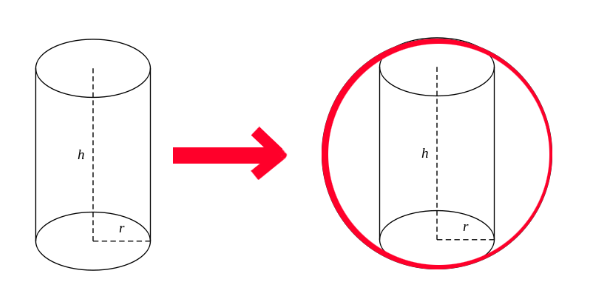
\includegraphics[width=13truecm, height=7.5truecm]{images/opt_5.1.png}
	\caption{Modell köré egy gömb alakú "hitbox" generálása}
	\label{fig:opt_1}
\end{figure}

\newpage
\Section{Távolság szűrése háromszögekkel}
Lényege, hogy ütközésvizsgálat előtt a modellek háromszögeinek a középpontját kiszámítjuk, majd a középpontokat viszonyítjuk egymáshoz, ahogy a \ref{fig:opt_2} ábrán láthatjuk. Ha a háromszögek közötti távolság nagyobb, mint a maximum táv, akkor az adott háromszög számítása elhanyagolható, mivel biztosra vehetjük, hogy nem lesz az adott két háromszög esetén metszés.

Az optimalizálás ezen esetben \textbf{sikertelen}, a számítások ideje drasztikusan megnő, használata nem ajánlott.

\Section{Távolság szűrése háromszögek mentésével}
Lényege ugyan az, mint az előző szekcióban bemutatott algoritmusnak, annyi kivétellel, hogy a középpontokat csak a modell beolvasásakor számítjuk ki, majd lementjük későbbi használatra, ahogy a \ref{fig:opt_2} ábrán láthatjuk.

Az optimalizálás ezen esetben \textbf{sikertelen}, a számítások ideje megnő az alaphoz képest, de csökken az előző algoritmushoz képest, illetve megnő a memóriaigény is. Használata nem ajánlott.
\begin{figure}[h]
	\centering
	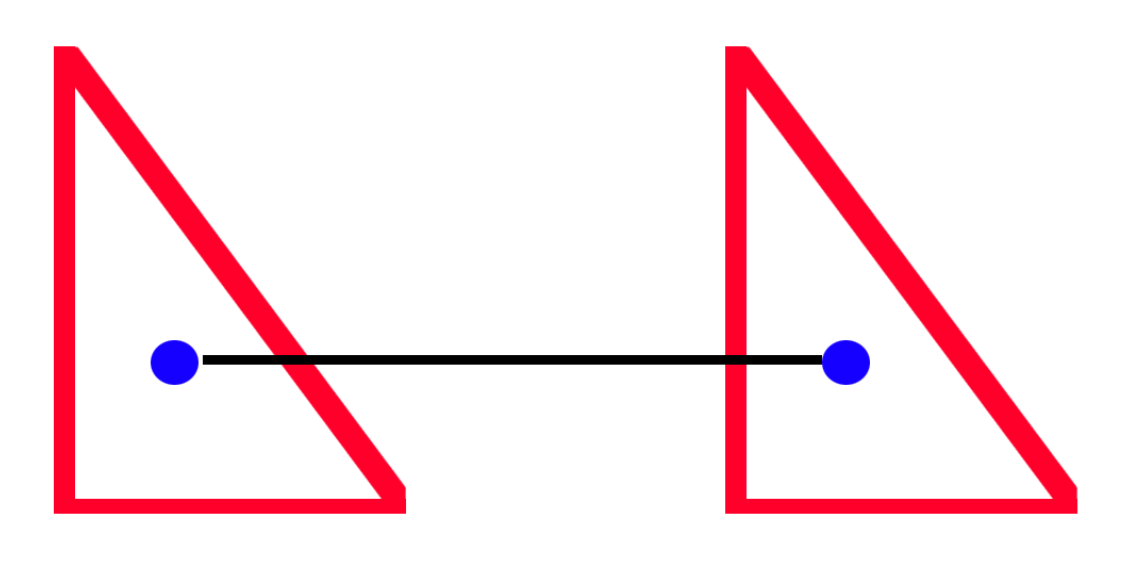
\includegraphics[width=13truecm, height=7.5truecm]{images/opt_5.2.png}
	\caption{Távolság szűrése háromszögek középpontjával}
	\label{fig:opt_2}
\end{figure}

\newpage
\Section{Pozíció alapján szűrés}
Lényege, hogy az adott modell nem feltétlenül van mindig ugyan abban a síkban, mint a másik vizsgálandó modell. Megnézzük a két modell középpontjának koordinátáit, illetve a legtávolabbi pontját az adott tengelyhez képest, ahogy a \ref{fig:opt_3} ábrán láthatjuk. Például ha a playermodellünk a Z koordinátán 20 cm magas, akkor a maximum szint a Z tengelyen az a modell középpontja + 20 cm lesz, minden más háromszöget az adott modellben figyelmen kívül hagyunk. Ezeket a lépéseket meg kell ismételnünk minden tengelyre 2 alkalommal. Ez összesen 6 különböző számítást jelent.

Az optimalizálás ezen esetben \textbf{megoldható}, a számítások ideje csökken, viszont programozás terén nehezen kivitelezhető, sok esetben hibákhoz vezethet, a memória igény nő.
\begin{figure}[h]
	\centering
	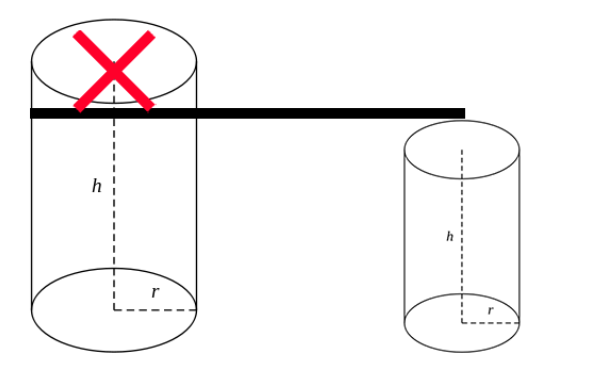
\includegraphics[width=13truecm, height=7.5truecm]{images/opt_5.3.png}
	\caption{Tengelyek alapján szűrés}
	\label{fig:opt_3}
\end{figure}